\documentclass[11pt]{article}
\usepackage{preamble}

\bibliography{database}

\lhead{AST3310}
\chead{Term project 3: Modelling a Star}
\rhead{Bendik Samseth}
\lfoot{}
\cfoot{}
\rfoot{\fancyplain{}{\thepage}}

\title{Term project 3: Modelling a Star}
\author{Bendik \textsc{Samseth}}
\date{\today}
\begin{document}
  % make title page
\begin{titlepage}
  \newcommand{\HRule}{\rule{\linewidth}{0.5mm}}
  \center
  \textsc{\LARGE University of Oslo}\\[1.5cm]
  \textsc{\Large AST3310}\\[0.5cm]
  \textsc{\large Term Project 3}\\[0.5cm]
  \HRule \\[0.4cm]
  { \huge \bfseries Modelling a Star}\\[0.4cm]
  \HRule \\[1.5cm]
  \Large \emph{Written by:}\\
  Bendik \textsc{Samseth}\\[3cm]
  {\large \today}\\[3cm]
  \vfill
\end{titlepage}


  \tableofcontents
  \begin{abstract}

    In this report we include energy transport by convection into the
    numerical model from project 2. First, a brief derivation is
    given, followed by the actual implementation in C++. The final
    model is found to not fit very well when using the parameters of
    the Sun. However, adjusting the initial parameters, a quite
    good-looking final star is produced. The modelled star has higher
    surface density, and lower temperature, but otherwise it is quite
    close to the Sun-values. All source material related to this
    report, which is cited at the relevant points, can be found at the
    projects GitHub repository~\cite{github}.

  \end{abstract}
%\end{@twocolumnfalse}
%]
\pagebreak



\section{Introduction}

In this report we will build upon the numerical model of a star from project 2, now adding energy transport by convection. In the case of the Sun, convective energy transport dominates from about $0.7R_\odot$ out to the surface, making it quite significant when we want a model of a \emph{full} star. The physics in deriving the equations is a bit involved, but parts of it is given in the next section. When everything is implemented we will get the chance to actually compare are model to the whole Sun, and look at how well it turns out.


\section{Adding Convection}

Following form the last report, we know that the governing equations for a star is:

\begin{align}
  \pd{r}{m} &= \frac{ 1 }{ 4\pi r^2\rho }\label{eq:drdm}\\
  \pd{P}{m} &= - \frac{ Gm }{ 4\pi r^4 }\label{eq:dPdm}\\
  \pd{L}{m} &= \epsilon\label{eq:dLdm}\\
  \pd{T}{m} &= - \frac{ 3\kappa L }{ 256 \pi^2 \sigma r^4T^3 }\label{eq:dTdm}
\end{align}

Adding convective energy transport equates to changing the last equation. This is because the temperature gradient in Eq.~\eqref{eq:dTdm} is based on all the energy being moved out of the star through radiation. When convection kicks in, the temperature gradient will become smaller, because not all the energy needs to be transferred by radiation anymore.


\subsection{Deriving the new equation}

So, we want to find the new temperature gradient, including both convection and radiation. We still know that the total energy flux must be related to the luminosity:

\begin{align}
    F_R + F_C = \frac{L}{4\pi r^2}\label{eq:total-flux}
\end{align}

We still have the radiative flux, given as

\begin{align}
    F_R &= \frac{4acGmT^4}{3\kappa P r^2}\nabla \label{eq:radiative-flux}
\end{align}

where $\nabla$ is the temperature gradient defined by $\nabla = \partial\ln T/\partial\ln P$.
We get Eq.~\eqref{eq:dTdm} by setting $F_C = 0$ and inserting into Eq.~\eqref{eq:total-flux}. Alternatively, we can solve for $\nabla$ and get

\begin{align}
    \nabla_{rad} = \frac{3\kappa L P} {64\pi\sigma G T^4 m}\label{eq:nabla-rad}
\end{align}

The subscript $\nabla_{rad}$ indicates that this is the temperature gradient we would have/need if all the flux is radiative.

This time, we are not setting $F_C = 0$, obviously, so what should we set it to? The full derivation is given in~\cite{lecture-notes}, and is to involved to be repeated in this report. A quick summary will do.


To get started, we will define a couple of quantities:

\begin{align}
    \delta &= -\left( \pd{\ln \rho}{\ln T} \right)_P=1\label{eq:delta-def}\\
    H_P &= -P\pd{r}{P} = \frac{P r^2}{\rho Gm} \label{eq:Hp-def}\\
    \nabla &= \pd{\ln T}{\ln P} = -\frac{H_P}{T}\pd{T}{r}\label{eq:grad-def}.
\end{align}

where $\delta$ is a shorthand symbol\footnote{$\delta$ simplifies to 1 when we use the ideal gas law, see Appendix~\ref{app:nabla-ad}}, and $H_P$ is the pressure scale height\footnote{We get the expression for $H_P$ by using the assumption of hydrostatic equilibrium.}. 
We want an equation for $\nabla$, as this would give us the temperature gradient we seek.

Furthermore, it can be shown (derivation once again in~\cite{lecture-notes}) that

\begin{align}
    v &= \sqrt{\frac{g\delta l_m^2}{4H_P}}(\nabla - \nabla^*)^{1/2}\label{eq:v}\\
    F_C &= \rho c_P T\sqrt{g\delta}H_P^{-\frac{3}{2}}\left(\frac{l_m}{2}\right)^2 (\nabla - \nabla^*)^{3/2}\label{eq:Fc-expression}
\end{align}

where $l_m$ is a constant with unit length. $\nabla^*$ is the temperature gradient for the little parcel of gas moving through the surroundings in the star (the other symbols have their regular meaning). We only care about the actual $\nabla$, so we want to eliminate $\nabla^*$.

We can say that $F_C+F_R=F_{rad}$, meaning that the total flux from convection \emph{and} radiation is equal to the flux we would have if the temperature gradient was big enough for all energy to be moved by radiation (i.e. $\nabla_{rad}$). Let's insert our expressions.

\begin{align*}
    F_R + F_C &= \frac{4acGmT^4}{3\kappa P r^2}\nabla_{rad}\\
    F_C &= \frac{4acGmT^4}{3\kappa P r^2} (\nabla_{rad} - \nabla)\\
    (\nabla - \nabla^*)^{3/2} &= \frac{4acGmT^4}{3\kappa P r^2} \frac{(\nabla_{rad} - \nabla) }{\rho c_P T\sqrt{g\delta}H_P^{-\frac{3}{2}}}\\
    (\nabla - \nabla^*)^{3/2} &= \frac{64\sigma T^3}{3\kappa\rho^2 c_P l_m^2} \sqrt{\frac{H_P}{g\delta}} (\nabla_{rad} - \nabla) \\
    &\equiv \frac{U}{l_m^2} (\nabla_{rad} -\nabla)\numberthis\label{eq:5-8-answer}.
\end{align*}

where we have defined for convenience the constant $U$ (which represents an energy in this case):

\begin{align}
    U = \frac{64\sigma T^3}{3\kappa\rho^2 c_P} \sqrt{\frac{H_P}{g\delta}}\label{eq:U-def}.
\end{align}

To continue, we need to use one more magic formula~\cite[Eq. (5.69)]{lecture-notes},

\begin{align*}
    (\nabla^*-\nabla_{ad}) &= \frac{32\sigma T^3}{3\kappa \rho^2 c_p v}\frac{S}{dQ}(\nabla - \nabla^*) \\
    \equiv& \frac{32\sigma T^3}{3\kappa \rho^2 c_p v} l_m\,K (\nabla - \nabla^*)\numberthis\label{eq:5-69},
\end{align*}

where $K = S/l_m d Q$ is a geometric constant defined for convenience, and $\nabla_{ad}$ represent the temperature gradient we would have if we had an adiabatic expansion of the parcel. If we  assume that the parcel is a sphere with diameter $d=l_m$, the parcel has a cross section $Q$ and surface area $S$, and $K$ reduces to

\begin{align}
    K = \frac{S}{l_m d Q} = \frac{4\pi r_p^2}{l_m^2 \pi r_p^2} = \frac{4}{l_m^2}.\label{eq:K-def}
\end{align}

Now we insert Eq.~\eqref{eq:5-69}, combined with Eq.~\eqref{eq:v} into the following equation:

\begin{align*}
    &(\nabla^* - \nabla_{ad}) = (\nabla - \nabla_{ad}) - (\nabla - \nabla^*)\\
    &\frac{32\sigma T^3}{3\kappa \rho^2 c_p v} l_m K (\nabla - \nabla^*) = (\nabla - \nabla_{ad}) - (\nabla - \nabla^*)\\
    &(\nabla - \nabla^*)\left[UK(\nabla-\nabla^*)^{-1/2} + 1\right]= \nabla - \nabla_{ad}\\
    &\Rightarrow \xi^2 + UK \xi - (\nabla-\nabla_{ad}) = 0\\
    &\Leftrightarrow \nabla = \xi^2 + UK \xi + \nabla_{ad}
\end{align*}

where $\xi = (\nabla-\nabla^*)^{1/2}$.

What we have is now an expression for $\nabla$, given by $\xi$ and $\nabla_{ad}$. The latter we know, so we need to find $\xi$. We do this by inserting $\xi$ into Eq.~\eqref{eq:5-8-answer}:

\begin{align*}
    (\nabla-\nabla^*)^{3/2} = \xi^3 = \frac{U}{l_m^2}(\nabla_{rad} - \nabla)\\
    \xi^3 = \frac{U}{l_m^2}\left(\nabla_{rad}  - (\xi^2 + UK \xi + \nabla_{ad})  \right)\\
    \Leftrightarrow \xi^3 + \frac{U}{l_m^2}\left( \xi^2 + UK\xi - (\nabla_{rad} - \nabla_{ad})\right) = 0\numberthis\label{eq:xi-third-order}.
\end{align*}

Eq.~\eqref{eq:xi-third-order} is a third order equation in $\xi$, but all the other parameters are known, so we can in principle solve this equation, and thereby get an expression for the true temperature gradient $\nabla$.

So, the steps we need to take are:

\begin{enumerate}
    \item Solve Eq.~\eqref{eq:xi-third-order} to get $\xi$.
    \item Insert into $\nabla = \xi^2 + UK\xi + \nabla_{ad}$.
    \item Solve for the gradient with respect to mass:
    \begin{align}
        \nabla &= \frac{P}{T}\pd{T}{P} = \frac{P}{T}\pd{m}{P}\pd{T}{m}\\
        &= \frac{P}{T} \left(- \frac{4\pi r^4}{Gm}\right) \pd{T}{m}\\
        \Rightarrow \pd{T}{m} &= -\frac{GmT}{4\pi r^4 P}\nabla.
    \end{align}
\end{enumerate}

\subsection{Instability criterion}
\label{sub:Instability criterion}

For our code, we would like to know if convection is taking place (and we need to use the harder formula derived in the last section), or if we can just use the old Eq.~\eqref{eq:dTdm}.

Convection will start if the temperature gradient $\partial T/\partial r$ is not large enough to transport all the energy by radiation. We say this by the inequality $\pd{T}{r} < \left(\pd{T}{r}\right)_{ad}$, or equvalently

\begin{align}
    \nabla_{rad} > \nabla_{ad}\label{eq:instability-criterion}.
\end{align}


So, the code will check if this is the case, and if so, apply the convection formula.



\subsection{Implementing the new Equation}
\label{sub:Implementing the new Equation}

We are continuing to build on top of the code from project 2. The addition of convection is achieved by testing for instability at each step in the integration loop, and calculating the new $\partial T/\partial m$. The actual calculation code is listed in Appendix~\ref{app:Code of Convection Implementation}. This is function that gets called before the new parameter values are calculated. It will alter some of the input variables, given as references, depending on whether or not we have convection.

The first thing the code does is check the instability criterion, and continues in the case that it holds. Then we set up all the quantities needed to define Eq.~\eqref{eq:xi-third-order}. The symbols have the same variable name as in the derivation, and should be easy to follow.

We then call a separate function to solve it. This function~\cite[\texttt{include/thirdordersolver.hpp}]{github}, always puts the real root of the polynomial in the first index, so only this solution is used.

With $\xi$ calculated we backtrace to get $\nabla$, and at last $\partial T/ \partial m$. In addition some other quantities are set, to be used in plots that will be shown later.


This is really the only thing that has changed from project 2, at least in terms of the core of the model.

\section{Finding the Best Parameters}
\label{sec:Finding the Best Parameters}

\subsection{Using Values of the Sun}
\label{sub:Using Values of the Sun}

\begin{figure}
    \center
    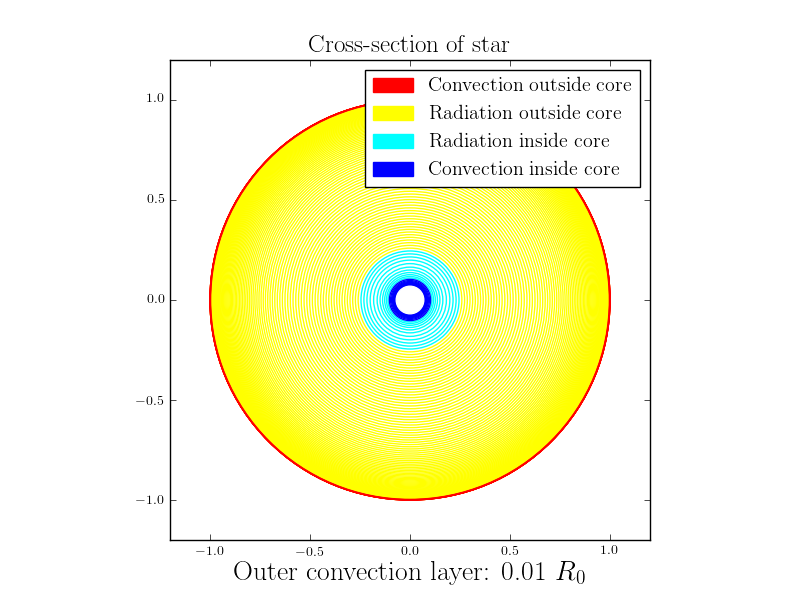
\includegraphics[width=\linewidth]{fig/cross_section_default.png}
    \caption{\label{fig:cross section default} The cross section of our star, given the values of the solar surface as initial parameters. We se a very thin outer convection zone, with radiation dominating essentially everywhere. }
\end{figure}

With the model developed, we can start to produce some results. A nice place to start could be to try the actual values for the surface of the Sun, since we are now modeling a full star.

Figure~\ref{fig:cross section default} shows the cross section of the resulting star. We see a very thin outer convection layer, followed by only radiation all the way in, with a small inner convection zone in the core. We se also that the integration didn't go all the way to $r=0$, because the solution became unphysical to fast. Obviously, this is not quite what we want, given that the Sun has about the outer $30\,\%$ as convection.

\subsection{Tweaking the Values}
\label{sub:Tweaking the Values}

We want to increase the size of the outer convection zone. This means that we want the instability criterion to take effect, meaning we want $\nabla_{rad}$ as large as possible. If we take a look at Eq.~\eqref{eq:nabla-rad}, we can see how $\nabla_{rad}$ depends on the other values. We have that

\begin{align*}
    \nabla_{rad} \propto \frac{P}{T^4} \propto \frac{\rho}{T^4}.
\end{align*}

This means that increasing the density and decreasing the temperature will make $\nabla_{rad}$ bigger, with the latter with a much stronger dependency.

Now that we know how to make $\nabla_{rad}$ bigger, we just have to find a balance that also keeps the solution acceptably close to completely physical (i.e. $r\rightarrow 0\Rightarrow L = m = 0$).

\subsection{Results with Best Model}
\label{sub:Results with Best Model}


After \emph{much} trial and error, I have landed on the following initial values:

\begin{align}
    \begin{split}
        &L_0 = L_\odot, R_0 = 1.1R_\odot,\ M_0 = 0.9M_\odot\\
        &\rho_0=80\rho_\odot,\ T_0 = 0.7 T_\odot,
    \end{split}\label{eq:best-param}
\end{align}
where $L_\odot, R_\odot, M_\odot$ and $T_\odot$ are all the solar values at the surface, and $\rho_\odot = \num{1.42e-7}\,\bar\rho_\odot$ with $\bar\rho_\odot$ as the average density of the Sun.

Before commenting on the results, I would like to preface this by saying that the exact ``best values'' are slightly arbitrary. Quite a large range of combinations give acceptable results, and why I landed on these values in particular are more by chance than I would like. There is, however, not a great way to score each set of values, because there are several factors that factors in to what makes an acceptable solution. At some point, I had to settle down on a set of values, and these happened to satisfy my requirements.


Now to the results. Figure~\ref{fig:main_params.png} show a plot of all the main parameters of the star. This is quite similar to the plots discussed in the previous project, so not much new to note. The main thing is that we can see that the core is about $20\%$ of the star ($L<0.995L_0$), and that both $L$ and $m$ is quite close to zero for $r\rightarrow 0$. For these parameters, the mass is about $4\%$ when the luminosity zeros out, so not perfect, but quite close.

Figure~\ref{fig:flux_fracs.png} shows the fractions of energy flux for radiation and convection. We see that convection dominates in the outer parts, but gets firmly put to zero further in the star.

Figure~\ref{fig:eps_fracs.png} show the fractions of energy being produced by the PPI and PPII cycles. We see, as we would hope, that PPI dominates for lower temperatures, while PPII takes over when $T$ gets large. Note that the first step, common to both cycles, is not included in this figure. This is because this term is very large in comparison to the other terms, making a comaprison very hard because the two cycles would seem almost identical. So the plot shows how the unique terms in the cycles compare. 

Finally, Figure~\ref{fig:cross_section_best.png} show the cross section using the new values. We see here once again that the outer convection zone is quite large, at $\sim 27\%$ of the total star. We can also see that radiation dominates for the rest of the star, and that the core is about $20\%$ of the radius. 

\subsubsection{Comparison with a Real Star}

We can compare the cross section in Figure~\ref{fig:cross_section_best.png} with the cross section of the Sun itself. Figure~\ref{fig:wiki-sun.png} shows an illustration taken from the main article of the Sun on Wikipedia. This is just an illustration, but it is drawn to scale, so we can in fact compare the two. I think, after all, that the result is quite comparable to this, which I will consider a success. We know that the Sun has a convection zone from about $0.7R_\odot$, which we is not to far off in the final model.  


\begin{figure}
    \center
    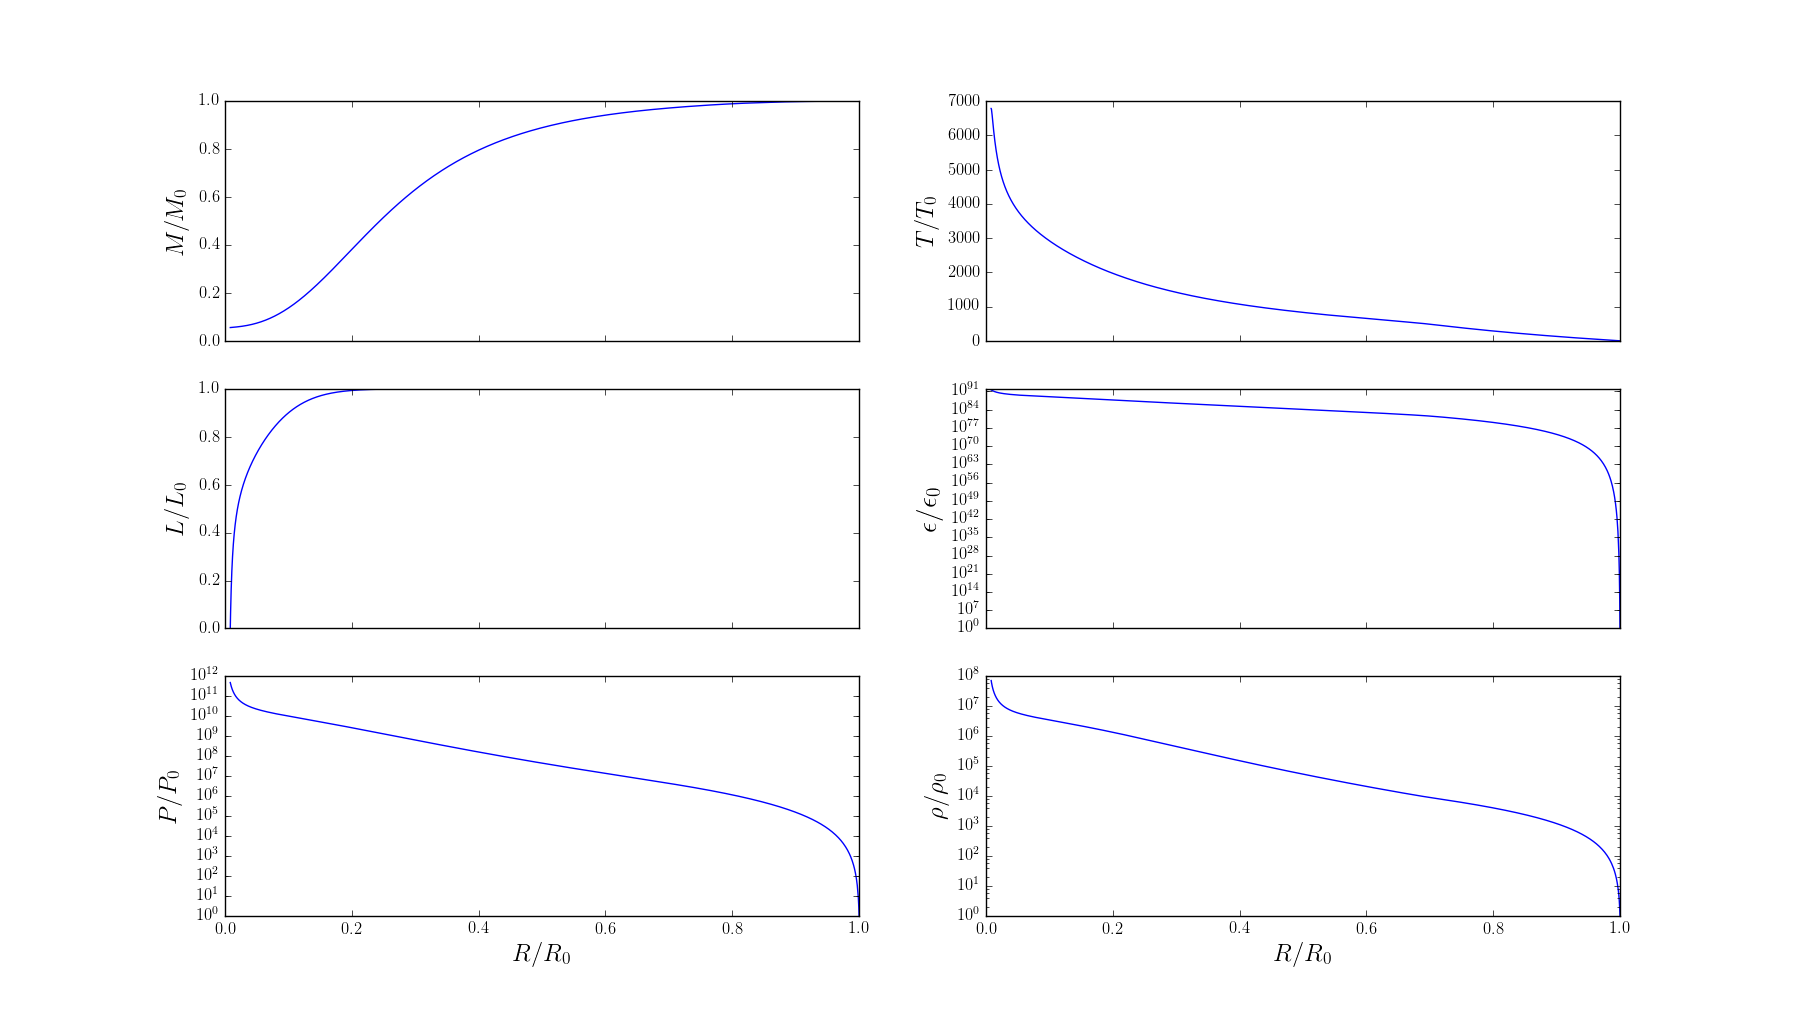
\includegraphics[width=\linewidth]{fig/main_params.png}
    \caption{\label{fig:main_params.png} The six main parameters of the star. We see a core of about $20\%$, and both $L$ and $m$ gets very close to zero for $r\rightarrow 0$. }
\end{figure}

\begin{figure}
    \center
    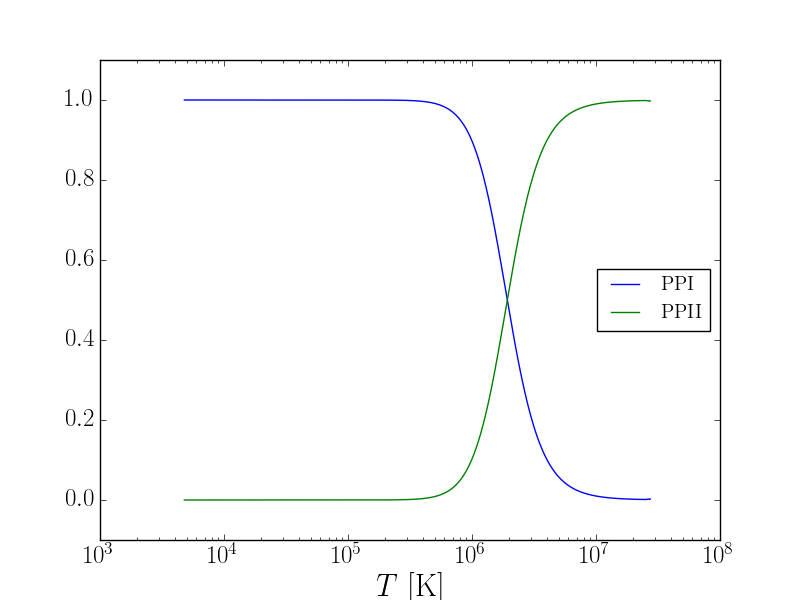
\includegraphics[width=\linewidth]{fig/eps_fracs.png}
    \caption{\label{fig:eps_fracs.png} The fractions of energy being produced by the PPI and PPII cycles. We se that PPI dominates for lower temperatures, while PPII catches up when $T$ gets sufficiently high.}
\end{figure}

\begin{figure}
    \center
    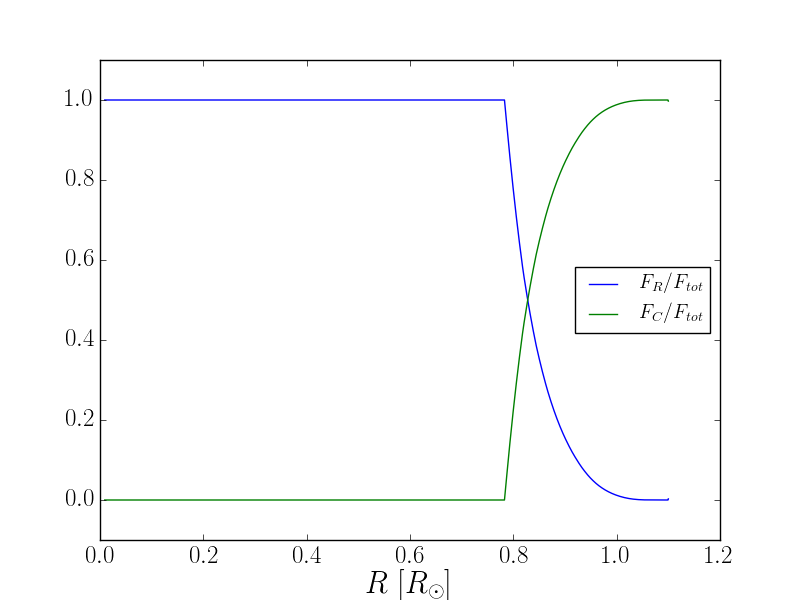
\includegraphics[width=\linewidth, height=0.4\textheight]{fig/flux_fracs.png}
    \caption{\label{fig:flux_fracs.png} The fractions of radiative- and convective flux. We se that convection dominates in the outer parts, but gets firmly put to zero further in the star.}
\end{figure}

\begin{figure}
  \centering
  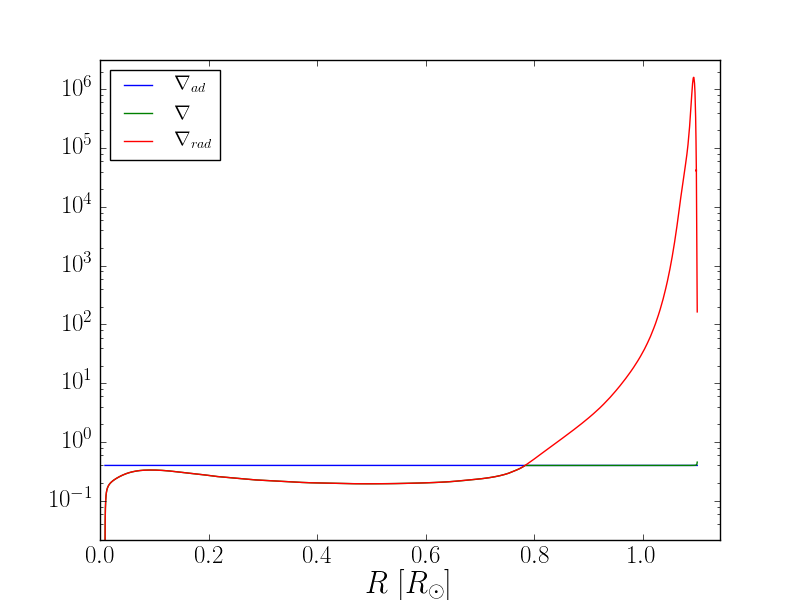
\includegraphics[width=\linewidth, height=0.4\textheight]{fig/nablas.png}
  \caption{\label{fig:nablas} The three temperature gradients $\nabla, \nabla_{rad}$ and $\nabla_{ad}$. We see $\nabla_{rad}$ going above the constant $\nabla_{ad}$ in the outer parts, in agreement with the size of the convection zone. $\nabla$ seems to be pretty much exactly equal to $\nabla_{ad}$ in these cases, and equal to $\nabla_{rad}$ (by definition) when smaller than $\nabla_{ad}$.}
\end{figure}

\begin{figure}
    \center
    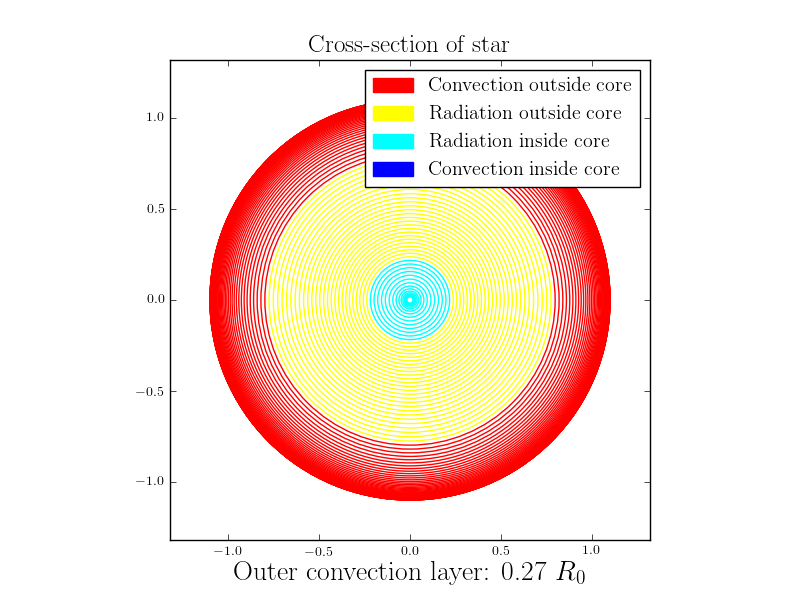
\includegraphics[width=\linewidth]{fig/cross_section_best.png}
    \caption{\label{fig:cross_section_best.png} Cross section of the star using the parameters in Eq.~\eqref{eq:best-param}. We have a sizable outer convection zone, and a decent sized core. In this model there is no inner convection layer.}
\end{figure}

\begin{figure}
    \center
    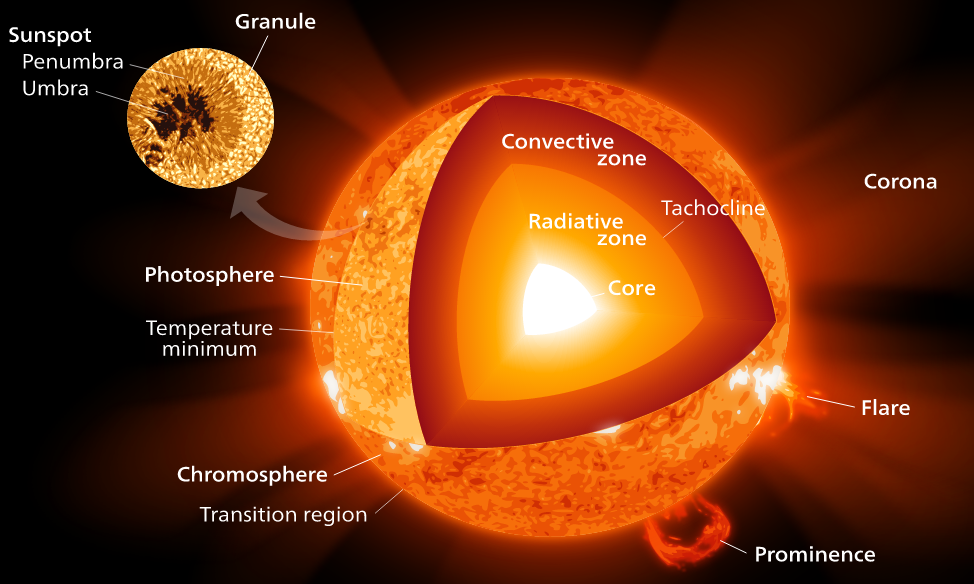
\includegraphics[width=\linewidth, height=0.3\textheight]{fig/wiki-sun.png}
    \caption{\label{fig:wiki-sun.png} Cross section of the Sun. Picture taken from Wikipedia, the main article for the Sun. Although not very quantitative, it is drawn to scale, so we can compare it to Figure~\ref{fig:cross_section_best.png}.}
\end{figure}


\pagebreak
\begin{appendices}
    \section{Calculating the Specific Heat for an Ideal Gas}
    In the following derivation, all lowercase quantities are per mass, unless otherwise stated.

    \subsection{Specific Heat at Constant Volume}
By definition, the specific heat at constant volume is:
\begin{align}
    dq &= c_v\,dT\hspace{0.5cm}(\text{constant volume})\label{eq:c_v-def}
\end{align}
Using the first law of thermodynamics, for constant volume, we get
\begin{align*}
    du &+ \frac{P\,dV}{m} = dq = c_v\,dT\\
    \Rightarrow c_v &= \frac{du}{dT}\numberthis\label{eq:c_v-expr}
\end{align*}

We find $u$ by using the equipartition theorem for a monoatomic, ideal gas. This gas has three degrees of freedom, so we get

\begin{align}
    u = \frac{3}{2}kT\cdot \frac{N}{m} = \frac{3}{2}kT\, \frac{1}{\mu m_u}\label{eq:u-equi}
\end{align}

Putting the last two equations together we get

\begin{align}
    c_v &= \frac{du}{dT} = \frac{3}{2} \frac{k}{\mu m_u}\label{eq:c-v-final}
\end{align}




\subsection{Specific Heat at Constant Pressure}
By definition, the specific heat at constant pressure is:
\begin{align}
    dq &= c_p\,dT\hspace{0.5cm}(\text{constant pressure})\label{eq:c_p-def}
\end{align}

We now remind our selfs of the ideal gas law, including the differential at constant pressure:

\begin{align}
    PV = NkT \Rightarrow P\,dV = Nk\,dT\label{eq:ideal-gas-diff}
\end{align}

We will use this in conjunction with the first law of thermodynamics:

\begin{align*}
    du &+ \frac{P\,dV}{m} = dq = c_p\,dT\\
    \Rightarrow c_p &= \frac{du}{dT} + \frac{Nk}{m} = \frac{du}{dT} + \frac{k}{\mu m_u}\\
    &= c_v + \frac{k}{\mu m_u}\numberthis\label{eq:c_v-c_p-rel}
\end{align*}

Finally, we insert the result from the last section:

\begin{align}
    c_p = \frac{5}{2} \frac{k}{\mu m_u}.\label{eq:c-p-final}
\end{align}



\section{Calculating the Adiabatic Temperature Gradient}
\label{app:nabla-ad}

The adiabatic temperature gradient is defined as follows:

\begin{align}
    \nabla_{ad} = \left(\pd{\ln T}{\ln P}\right)_{ad}\label{eq:nabla_ad-def}
\end{align}

It can be shown that this can be expressed as~\cite[Eq. (5.40)]{lecture-notes}

\begin{align}
    \nabla_{ad} = \frac{P\delta}{T\rho c_p}\label{eq:nabla_ad-expr}
\end{align}

The factor $\delta$ is defined in Eq.~\eqref{eq:delta-def}, and can be simplified significantly by using the ideal gas law. We write this up once more, this time with the density $\rho$:

\begin{align}
    P = \frac{\rho kT}{\mu m_u}\label{eq:ideal-gas-rho-def}
\end{align}

We then have

\begin{align*}
    \delta &= -\frac{T}{\rho}\pd{\rho}{T} = -\frac{T}{\rho}\left(-\frac{P\mu m_u}{kT}\frac{1}{T^2}\right)\\
    &= \frac{P\mu m_u}{\rho kT} = \frac{\rho kT}{\mu m_u} \frac{\mu m_u}{\rho kT}\\
    &= 1
\end{align*}

Now we get the adiabatic temperature gradient by applying Eq.~\eqref{eq:ideal-gas-rho-def} to Eq.~\eqref{eq:nabla_ad-expr}, along with the result for $c_p$ from the previous section:

\begin{align*}
    \nabla_{ad} &= \frac{P\delta}{T\rho c_p} = \frac{\rho kT}{\mu m_u} \frac{1}{T\rho c_p}\\
    &= \frac{k}{\mu m_u} \, \frac{2}{5}\frac{\mu m_u}{k} \\&= \frac{2}{5}
\end{align*}

\pagebreak
\section{Code of Convection Implementation}
\label{app:Code of Convection Implementation}

\lstinputlisting[basicstyle=\footnotesize, language=C++, firstline=28, lastline=75]{../src/integrate.cpp}


\end{appendices}

\printbibliography
\end{document}

%%% Local Variables:
%%% mode: latex
%%% TeX-master: t
%%% End:
